\documentclass[a6paper]{article}
% Lets us set the author and title of the compiled pdf file
\usepackage[pdftex]{hyperref}

% Lets make the text nice and big
\usepackage[14pt]{extsizes}


% Have a header and footer to keep the page sizes constant on the kindle
\usepackage{fancyhdr}

% Make the borders really small
\usepackage[left=0.3cm,
      top=1cm,
      right=0.2cm,
      bottom=0.2cm,
      marginparwidth=0mm,
      marginparsep=0mm]{geometry}

% Import the packages for the notes
% Tell me about my LaTeX bad practices
\usepackage[l2tabu, orthodox]{nag}
% For \hypersetup
\usepackage{hyperref}
% For line brakes in tables
\usepackage{tabularx}
% For the split environment
\usepackage{amsmath}
\usepackage{amssymb}
% For tabs in verbatim
\usepackage{moreverb}
% For images
\usepackage{graphicx}
% Side by side figures
\usepackage{subcaption}
% For code listings
\usepackage{listings}
% For wrapping figures
\usepackage{wrapfig}
% For exact placement of floats
\usepackage{float}
% For fancy verbatim (use this one in mymulticol)
\usepackage{alltt}
% For splitting long lists into columns
\usepackage{multicol}
% Multi rows..
\usepackage{multirow}
% For no multicol on the kindle
\usepackage{environ}
\newif\ifmulticols
\NewEnviron{mymulticols}{
\ifmulticols
  \begin{multicols}{2}
    \BODY
  \end{multicols}
\else
  \BODY
\fi}
% Means you don't have to put \\ to start a new line.
\usepackage[parfill]{parskip}
% Make LaTeX pretty with better kerning etc
\usepackage{microtype}

% If enabled, maybe skip certain stuff or do it for less time to compile faster
\ifdefined\fastCompile
  % Fast param here:
  % \newcommand{\samplesScaleFactor}{0.1}
\else
  % Slow param here:
  % \newcommand{\samplesScaleFactor}{1.0}
\fi

% Make a box around would-be margin paragraphs
\usepackage{tcolorbox}

% Set the tab size in verbatim to 1
\def\verbatimtabsize{1\relax}

% Make margin paragrahs inline
\renewcommand{\marginpar}[1]{
\begin{tcolorbox}[colback=white!5,colframe=white!40!black,title=Note:]
#1
\end{tcolorbox}}

\begin{document}

% No page numbers!
\pagenumbering{gobble}

% Get the author, the title etc
% Set the info about the notes
\newcommand{\coursename}{Compilers}
\newcommand{\coursecode}{COMP36512}
\newcommand{\courseinfo}{\section*{Overview}

This course will explore certain classes of algorithms for modelling and
analysing complex systems, as arising in nature and engineering. These examples
include: flocking algorithms - e.g., how schools of fish or flocks of birds
synchronised; optimisation algorithms; stability and accuracy in numerical
algorithms.

\section*{Aims}

By the end of the course, students should:
\begin{itemize}
\item Be able to apply what they learnt across different disciplines.
\item Appreciate the emergence of complex behaviours in networks not present in
the individual network elements.
\end{itemize}

\section*{Syllabus}

\begin{mymulticols}
    \begin{itemize}
    \item PART 1: NUMERICAL STABILITY AND ACCURACY OF COMPUTATIONS (10 hours)
      \begin{itemize}
        \item Introduction to finite precision computation (2 hours)
        \item Floating point arithmetic (examples that include error analysis insummation, evaluation of polynomials, recurrences, and basic linear algebra)(3 hours)
        \item Mixed precision algorithms (basic concept of iterative refinement,different speed of execution on different architectures, linear algebraexamples) (1 hour)
        \item Numerical solution of initial value problems (explicit/implicit methods,multistep methods, consistency, stability, convergence) (2 hours)
        \item Find the equilibria of a dynamical system, and analyse the stability of said system (2 hours) \\ \newline
      \end{itemize}

  \item PART 2: COMPLEX NETWORKS AND COLLECTIVE BEHAVIOUR (8 hours)
    \begin{itemize}
      \item Complex networks are groups of systems (normally, a big number of them) interconnected in a non-trivial and non-regular way
Introduction to complex networks (2 hours)
	Where are the networks and the complexity?
	Characterisation of complex networks
	Basic network properties and terminology. Topological analysis
      \item Complex network models. The structure of the network (2 hours)
	Regular networks
	Random-graph networks
	Small-world networks
	Scale-free networks
      \item Network dynamics and collective behaviour (3 hours)
	Distributed/local versus centralised/global
	The concept of self-organisation
	Synchronisation in complex dynamical networks
	Consensus over complex networks
	Swarm dynamics
	Consensus protocols
	Flocking algorithms
        \end{itemize}
  \end{itemize}
\end{mymulticols}

\section*{Attribution}

These notes are based off of both the course notes (found on
Blackboard). Thanks to the course staff (Eva Navarro-Lopez, Milan
Mihajlovic and Pedro Mendes) for such a good course! If you find any
errors, then I'd love to hear about them.

\section*{Contribution}

Pull requests are very welcome:
\url{https://github.com/Todd-Davies/third-year-notes}
}
% Set the author and title
\newcommand{\Author}{Todd Davies} 
\newcommand{\Title}{Compilers}
% Meta
\author{\Author}
\title{\Title}


\pagestyle{fancy}% Change page style to fancy

\fancyhf{}% Clear header/footer
\fancyhead[C]{}
\fancyfoot[C]{}
\renewcommand{\headrulewidth}{0.01pt}
\renewcommand{\footrulewidth}{0.01pt}

\maketitle

% Get the course info
\courseinfo
\newpage

% Table of contents
\tableofcontents
\newpage

% Don't do multicol
\multicolsfalse

% Get the content of the file
% Set the author and title of the compiled pdf
\hypersetup{
  pdftitle = {\Title},
  pdfauthor = {\Author}
}

\section{Algorithmic Wisdom}

{\hspace{2.2em} \small Lectures 2 \& 3}

The first two lectures of the course describe different types of algorithms,
what is computable, where to optimise algorithms, asymptotics and heuristics.

\subsection{Different types of algorithms}

There are three types of algorithms that are mentioned:

\marginpar{You should know all of this from \texttt{COMP26120}.}

\begin{description}
  \item \textbf{Divide and conquer}\\
  These algorithms continually break a problem down into smaller parts, which
  are easier to solve, until eventually, the problems are trivial and easily
  solved. This is often used when the data you're operating on is in a
  recursive datastructure such as a tree. If you're writing an algorithm to
  find how many nodes there are in a tree, then you could use divide and
  conquer:

  \begin{lstlisting}[language=java]
    int countTreeSize(tree) {
    int size = 1;
    if (tree.left) size += countTreeSize(tree.left);
    if (tree.right) size += countTreeSize(tree.right);
    return size;
    }
  \end{lstlisting}

  As you can see from the example, divide and conquer algorithms are usually
  recursive.

  The divide and conquer technique can be applied to graphs, but in order to
  do this, you must keep track of which nodes you've visited with a flag on
  each node. If we wanted to count the nodes in a graph, we could do:

  \begin{lstlisting}[language=java]
    int countGraphSize(graph) {
    if (graph.visited) return 0;
    graph.visited = true;
    int size = 1;
    for (child in graph) {
      size += countGraphSize(child);
    }
    return size;
    }
  \end{lstlisting}

  \item \textbf{Mutual Recursion}\\
  Mutual recursion describes an algorithm that operates on data where one type
  of data can reference another, and the other can reference it. The example
  given is that of statements and expressions in programming languages;
  statements contain expressions, and expressions can also contain statements.
  Parsing such a structure might involve two algorithms that recurse on each
  other!

  \item \textbf{Dynamic Programming}\\
  Dynamic programming exploits the fact that when some problems are broken
  down into smaller sub-problems, some of the sub-problems are identical.
  Dynamic programming algorithms start from the very smallest sub-problems and
  build up to the final solution, and usually cache results to sub-problems in
  a table so that work is not done twice.

\end{description}

\subsection{Computability}
% TODO: Combine this with a later topic?

There are many different definitions of computability, including
\href{https://en.wikipedia.org/wiki/Lambda_calculus}{lambda calculus},
\href{https://en.wikipedia.org/wiki/Turing_machine}{Turing machines},
\href{https://en.wikipedia.org/wiki/Rewriting}{rewriting rules},
\href{https://en.wikipedia.org/wiki/Random-access_machine}{random access
machines} and (many) more. The idea that relates all of these things, is that
they all have the same capabilities. That is to say that if you can compute
something using one of these ideas, then you can also compute it on all the
others too.

There are also a class of `alternate' computing mechanisms, such as quantum
computers and neural computers. These ideas have the potential to compute things
that a Turing machine (or its equivalents cannot), but they are significantly
harder to build, and functional implementations do not exist yet.

\subsection{Asymptotics and optimisation}

When you have to get a computer to perform a task, implementing a simple
algorithm first is a good idea, since you will at least have something to
demonstrate to people, and you will gain a good understanding of the problem at
hand. However, simple algorithms are often slow; how should we evolve our
implementation to be as fast as we need it to be?

Profiling can tell you where your code is spending most of its time. Sometimes
your algorithm will be really fast, and the processor will spend most of its
time waiting for IO to give it more data; this is often the case with GPU
computation.

Assuming you find some CPU bottleneck in your code, before you spend hours
making it faster, consider whether it is worth the effort. If this part takes up
10\% of your runtime, and you make it twice as fast, your program will only run
5\% faster. This is an example of the
\href{https://en.wikipedia.org/wiki/Diminishing_returns}{Law of Diminishing
Returns}.

As well as optimising specific parts of an algorithm, you also should consider
its asymptotic run time. An algorithm that runs in $O(n^2)$ time is probably
going to be better than one that runs in $O(n log(n))$ time. However, this isn't
always the case; some algorithms (often ones with good asymptotic run times)
take a long time to set up, usually when you have to transform the data into
some different datastructure. If you are running your algorithm on a small
amount of data, then an algorithm that you can run on your data \textit{as is}
might outperform a fancier algorithm that you have to invest more overhead in.

\marginpar{Sometimes a good solution is to use different algorithms depending
on the input. If there are only a few cases that produce worst-case performance,
you could even hard-code solutions to those!}

The average case runtime of a algorithm is also important. Haskell uses a type
checker that runs in $O(2^{n^n})$ time in the worst case, but for every program
that isn't made specifically to mess with the compiler, runs in linear time.

\section{Graphs}

A graph is a pair $G = (V,E)$ where $V$ is a finite set, and $E$ is a set of
pairs between items in $V$. Elements in $V$ are \textit{vertices} or
\textit{nodes}, and elements in $E$ are \textit{edges}.

Different mathematicians have different rules about what exactly can go in a
graph. For the purposes of this course, the graphs shown in
Figure~\ref{fig:bad-graphs} aren't allowed.

\begin{figure}[h]
  \centering
  
\includegraphics{diagrams/self-loops}\\
  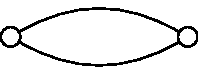
\includegraphics{diagrams/multiple-edges}\\
  
\includegraphics{diagrams/directed-graph}
  \caption{Self loops, duplicate edges and arrows are not allowed.}
  \label{fig:bad-graphs}
\end{figure}

A \textbf{directed graph} is just like a normal graph, except the edges do have
arrows. The only mathematical difference is that the set $E$ is a set of ordered
pairs.

The \textit{degree} of a node in a graph, is the number of edges that are
adjacent to (touching) it. If the graph is directed, then it is the number of
edges originating from the node.

A weighted graph is one where each edge is associated with a value representing
its weight. The length of a path between nodes is simply the sum of the edge
weights connecting the nodes.

\subsection{Connectivity}
\label{connectivity}

A node $a$ is \textbf{reachable} from another node $b$ if there is some sequence
of nodes connected by edges that go from the $a$ to $b$.

A graph where every node is reachable from every other node is
\textbf{connected}. A strongly connected graph is a \textbf{directed graph}
where each node is reachable from each other node.

\begin{figure}[h]
  \centering
  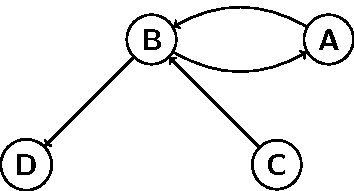
\includegraphics{diagrams/connected-graph}
  \caption{This graph is not strongly connected, but the subgraph with only
  nodes $A$ and $B$ is. If we were to remove the arrows, then the graph would
  be connected.}
  \label{fig:connected-graph}
\end{figure}

\subsection{Representing graphs}

We can store graphs in computer memory in two ways:

\begin{description}
  \item \textbf{Adjacency List}\\
    There are two different kinds of adjacency list, the first is like so:

    \begin{lstlisting}[language=java]
      public class Graph {
        List<Vertex> nodes;
        List<Edge> edges;
      }
      public class Edge { Vertex a, b; }
      public class Vertex { List<Edge> outlist; }
    \end{lstlisting}

    Here, we keep a list of all the nodes, and a list of all the edges. From
    any edge, we can see what nodes it connects, and from any node, we can
    see what edges it connects.

    The other type of adjacency list is a bit simpler, but less efficient in
    some cases:

    \begin{lstlisting}[language=java]
      public class Graph<T> {
        Set<T, List<T>> adjList;
      }
    \end{lstlisting}
  \item \textbf{Adjacency Matrix}\\
    Here, a matrix indicates whether there is an edge between two nodes:

    \begin{center}
      \begin{tabular}{c|c c c c}
          & A & B & C & D\\ \hline
        A & 0 & 1 & 0 & 0\\
        B & 1 & 0 & 0 & 1\\
        C & 0 & 1 & 0 & 0\\
        D & 0 & 0 & 0 & 0\\
      \end{tabular}
    \end{center}

    This adjacency matrix represents the graph in
    Figure~\ref{fig:connected-graph}. You can see that it is fairly wasteful
    in terms of memory $O(|E|* |V|)$, though with bit arrays, it has a very 
    low constant overhead.
\end{description}

\subsection{Classifying Edges}

During a \textit{depth first traversal} (Section~\ref{depth-first-search}) of a
graph, we can classify each edge into one of four types. When doing the
traversal, we process each edge from left to right (from the viewer's
perspective), and we define an edge to be an \textit{ancestor} of another edge
if there is a path from the ancestor edge to the descendent edge and the ancestor
is traversed first. The four types of edges are:

\begin{description}
  \item \textbf{Tree edges}\\
    These edges lead to a new node during a search. If you remove all the edges 
    from the graph except tree edges, then you get a tree!
  \item \textbf{Forward edges}\\
    These go from ancestor edges to descendent edges, but are not tree edges
    (i.e. the descendent node has been visited already).
  \item \textbf{Cross edges}\\
    These go between edges where no node is the ancestor of the other.
  \item \textbf{Back edges}\\
    An edge that goes from a descendant to an ancestor.
\end{description}

\begin{figure}[h]
  \centering
  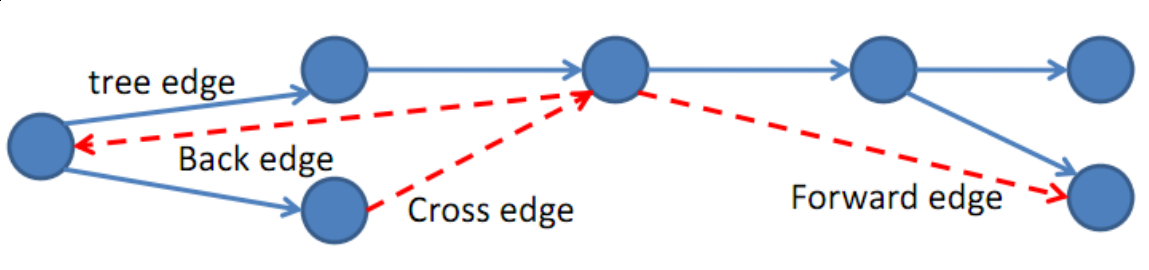
\includegraphics[width=0.6\textwidth]{images/edge-types}
  \caption{A
  \href{http://courses.csail.mit.edu/6.006/spring11/rec/rec13.pdf}{pictorial
  illustration} of the different edge types.}
  \label{fig:connected-graph}
\end{figure}

\subsection{Graph Algorithms}

You will have covered some of the algorithms featuring here in previous courses,
or perhaps seen them in the wild. They are however interesting and useful, so
it's worth a recap even if they're not new! I've ordered these in roughly
increasing order of mental strain.

\subsubsection{Depth first search}
\label{depth-first-search}

\href{https://en.wikipedia.org/wiki/Depth-first_search}{Depth first search}
(DFS) is an algorithm to find a node in a graph starting from another node. It
works on both directed and undirected graphs, and runs in $O(|V| + |E|)$
(linear) time. The psudo code looks like this:

\marginpar{Note how we mark nodes as having been visited (by adding them to
\texttt{visitedNodes}). This is so if there is a loop in the graph, the 
algorithm doesn't run indefinitely.}

\begin{lstlisting}[language=java]
  Node dfs(Node haystack, Node needle) {
    Stack<Node> toVisit = new Stack<>();
    Set<Node> visitedNodes = new Set<>();
    toVisit.push(haystack);
    while(!toVisit.isEmpty()) {
      Node node = toVisit.pop();
      if (visitedNodes.contains(node)) continue;
      visitedNodes.add(node);
      if(node.equals(needle)) {
        return needle;
      } else {
        for(Node child : node.children) {
          toVisit.push(child);
        }
      }
    }
    return null;
  }
\end{lstlisting}

A Breadth First Search is the same, except you use a \texttt{Queue} instead of a
\texttt{Stack}.

\marginpar{To see if a graph is connected, do a depth first search as in the
example code, but don't stop when you find a needle, only stop when the
\texttt{toVisit} stack is empty. If \texttt{visitedNodes} contains all of the
nodes in the graph, then the graph is connected.}

Depth first search also lets you find if one node is reachable from another in
linear time, and also if a graph is connected in linear time too, with a few
modifications.

We can also find out if a directed graph is strongly connected in $O(|V| + |E|)$
time using Tarjan's algorithm, which we'll see later.

\subsubsection{Dijkstra's algorithm}

Dijkstra's algorithm finds the undirected shortest path between two nodes in a
graph. Here is the psudo-code:

\marginpar{My best advice for learning an algorithm like this, is to get a 
whiteboard, draw out the problem, and then run the solution manually on the 
whiteboard. Then you have a pictorial and visual explanation of how the 
algorithm \textit{really} works.}

\begin{lstlisting}[language=java,
                  caption=Dijkstra's algorithm (from Wikipedia),
                  label=lst:dijkstra,
                  captionpos=b]
function Dijkstra(Graph, source):
  create vertex set Q

  // Initialization
  for each vertex v in Graph:
    dist[v] = INFINITY
    prev[v] = UNDEFINED
    add v to Q

  // Distance from source to source
  dist[source] = 0

  while Q is not empty:
    u = vertex in Q with min dist[u]
    remove u from Q 

  for each neighbour v of u:
    alt = dist[u] + length(u, v)
    // A shorter path to v has been found
    if alt < dist[v]:
      dist[v] = alt 
      prev[v] = u 

  return dist[], prev[]
\end{lstlisting}

If we use a Fibonacci heap, for the priority queue, then the runtime of
Dijkstra's algorithm is $O(|E| + |V|log(|V|)$. If we use a normal heap, then the
runtime is $O(|E|log(|V|))$.

\subsubsection{Tarjan's Algorithm}

Before we delve into Tarjan's Algorithm, we need to discuss strongly connected
components. You will remember from Section~\ref{connectivity}, that a graph is
strongly connected if all nodes are reachable from any other node.

A \textit{strongly connected component} is a subset of edges within a graph,
where the subset is strongly connected. If a graph has only one strongly
connected component, then it is strongly connected.

The psudo code here is from
\href{https://en.wikipedia.org/wiki/Tarjan%27s_strongly_connected_components_algorithm}{Wikipedia}.
If you're reading this after week 8 of the \texttt{COMP36111} course, then you
probably have your own implementation in C.

\begin{lstlisting}
  algorithm tarjan is
  input: graph G = (V, E)
  output: set of strongly connected components (sets of vertices)

  index := 0
  S := empty
  for each v in V do
    if (v.index is undefined) then
      strongconnect(v)
    end if
  end for

  function strongconnect(v)
    // Set the depth index for v to the smallest unused index
    v.index := index
    v.lowlink := index
    index := index + 1
    S.push(v)
    v.onStack := true

    // Consider successors of v
    for each (v, w) in E do
      if (w.index is undefined) then
        // Successor w has not yet been visited; recurse on it
        strongconnect(w)
        v.lowlink  := min(v.lowlink, w.lowlink)
      else if (w.onStack) then
        // Successor w is in stack S and hence in the current SCC
        v.lowlink  := min(v.lowlink, w.index)
      end if
    end for

    // If v is a root node, pop the stack and generate an SCC
    if (v.lowlink = v.index) then
      start a new strongly connected component
      repeat
        w := S.pop()
        w.onStack := false
        add w to current strongly connected component
      while (w != v)
      output the current strongly connected component
    end if
  end function
\end{lstlisting}

%TODO: Expand on Tarjan's algorithm when a whiteboard is present

\section{Linear Programming}

Linear programming is an optimisation problem, where we want to find the `best'
solution to a set of equations. We're going to solve it using the
\textit{simplex} method, but before we do, I think it's a good idea to recap
some high-school mathematics first. Feel free to skip the next subsection if
you're feeling confident with it.

\subsection{Background mathematics}

An inequality relation is just like a normal equation, except the equals sign is
replaced by either $<$, $>$, $\leq$ or $\geq$. When you solve an inequality, you
generally want to get all of the similar terms on one side (e.g. move all the
variable terms over to one side, and all of the constants to another side). This
\textit{mostly} works like a normal equation; you can add and subtract from both
sides just like normal, however, if you want to divide or multiply \textbf{by a
negative quantity}, then you need to \textbf{reverse the equality}.

\[
  \begin{split}
    -2x &> -2\\
    2x &< 2\\
    x &< 1
  \end{split}
\]

This equality is satisfied whenever $x$ is less than $1$. If we have two terms
in the equality (something similar to $ax + by \geq c$), it becomes slightly
harder to solve. To solve this we can:

\begin{itemize}
  \item Plot a graph of the line $ax + by = c$.
  \item Pick a test point $(x, y)$ not on the line, and plot it on the graph.
  \item If the point $(x, y)$ satisfies the inequality, then shade the opposite 
    side of the line to which the point is on, otherwise, shade the same side.
\end{itemize}

For example, given $3x + 4y \leq 6$, and choosing the point $(-2,1)$ we end up
with what's in Figure~\ref{fig:graph-1}.

\begin{figure}[h]
  \centering
  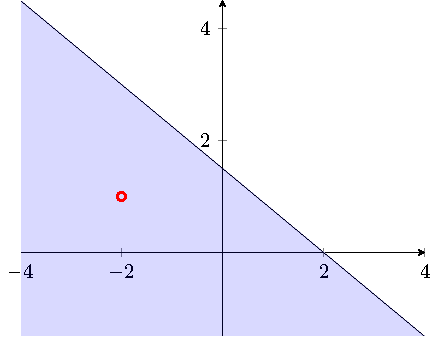
\includegraphics{diagrams/graph1}
  \caption{A graph of $3x + 4y \leq 6$, with all the valid values shaded blue.}
  \label{fig:graph-1}
\end{figure}

If we have multiple inequalities, we want to \textit{find the region where all
of them are satisfied}. This involves plotting each line, and shading the
regions where they're not satisfied, which means the blank bit is the bit we
want.

If we have the equations $3x + 4y \leq 6$, $2y - x \leq 2$ and $x \geq 0$, we
will get something like in Figure~\ref{fig:graph-2}.

\begin{figure}[h]
\captionsetup{width=.4\linewidth}
\centering
\begin{minipage}{.5\textwidth}
  \centering
  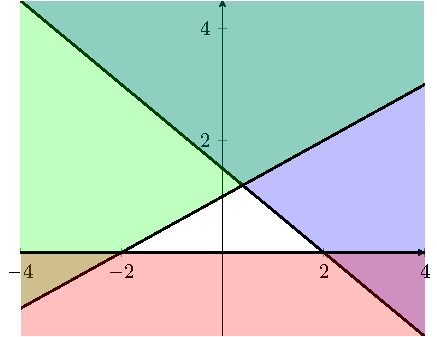
\includegraphics[width=.8\textwidth]{diagrams/graph2}
  \captionof{figure}{A graph plotting $3x + 4y \leq 6$, $2y - x \leq 2$ and
  $x \geq 0$, where the points not satisfying the inequalities are shaded in 
  blue, green and red respectively. The clear region satisfies all points.}
  \label{fig:graph-2}
\end{minipage}%
\begin{minipage}{.5\textwidth}
  \centering
  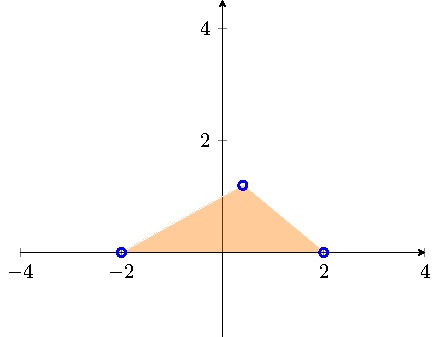
\includegraphics[width=.8\textwidth]{diagrams/graph3}
  \captionof{figure}{The valid region in the three inequalities from
  Figure~\ref{fig:graph-2}. The corner points are $(2,0),(-2,0)$ and
  $(\frac{2}{5},\frac{6}{5})$.}
  \label{fig:graph-3}
\end{minipage}
\end{figure}


The corner points are especially important to us, since that's often where the
useful numbers are (we'll see more of this later). In order to find the corner
points, we solve the two lines that form them. Solving the following equations
gives the points in Figure~\ref{fig:graph-3}.

\begin{mymulticols}
  \begin{itemize}
    \item $x = 0, 3x + 4y = 6$
    \item $x = 0, 2y - x = 2$
    \item $2y - x = 2, 3x + 4y = 6$
  \end{itemize}
\end{mymulticols}

% Up to 4.4 in the Linear Equalities booklet.

\end{document}